This chapter first outlines limitations of current approaches in the field of cooperative perception and motivates this work's contributions to overcome them. Second, goals and conceptual requirements are presented as a guideline for later system design. Finally, it is made clear which, aspects are in or out of scope of this thesis.

\section{Current Limitations}
\label{sec:problem_analysis:current_limitations}

Existing work in the field of cooperative perception, as presented in \autoref{ch:related_work}, faces several limitations.
\par
\bigskip

One of them is a \textbf{lack of comprehensiveness}. While the shown studies each focus on certain aspects of a CP system, to the best of our knowledge, no solution was presented that is both holistic and detailedly concerned with all individual parts of the system. Also, not all previous project provide an actual implementation of their proposal or do not conduct realistic simulations.
\par
\bigskip

Moreover, \textbf{no standardized, uniform, yet expressive environment model} and state representation for traffic scenes exists, yet. While the efforts taken by \cite{EuropeanTelecommunicationsStandardsInstituteETSI2019} to specify a standard for CPMs are promising, at this point, there is nothing like that available to be used in CP systems. Current models are either incomplete, proprietary and non-transparent ot not suitable for interoperability between heterogeneous systems. 
\par
\bigskip

Another significant issue arises from limitations regarding \textbf{scalability of VANET-based cooperative perception systems}.

One essential challenge is the limited \textbf{throughput}, \textbf{range} and minimum \textbf{latency} of DSRC networks, usually based on IEEE 802.11p technology. \cite{5GAutomotiveAssociation2018} found DSRC to be 90 \% reliable at 675 m distance between sender and receiver in line-of-sight scenarios and 375 m in non-line-of-sight situations. As a comparison, 5G showed 90 \% reliability at 1175 m and 875 m, respectively. Although the absolute results of these tests are debatable, as \cite{Mangel2011} found DSRC NLOS reception to be only 50 \% at 50 m distance, it is clear that 5G technology usually provides better performance. Measurements concerning maximum throughput with IEEE 802.11p range from 2.7 Mbps to 11 Mbps per channel. Average latency in typical CP use cases was measured to range from 3 ms to 22 ms by \cite{Rauch2011}.

Despite limited performance of DSRC, VANET-topology-based CP systems face another problem, which is related to \textbf{network utilization}. Many implementations of such networks implement complete pair-wise P2P connections among participants. Consequently, the number of connections is given as $N = \frac{n(n-1)}{2 }$ according to \textit{Metcalfe's law}. 

Due to these inherent restrictions of DSRC, recent publications tend to favor upcoming 5G technology \cite{Briegleb2019, 5GAutomotiveAssociation2016}, e.g. \cite{Wevers2017} claims that \textit{"'development of V2X services in 5G makes much sense, and holds promises for the future"'}.

A more detailed comparison between DSRC and 5G is presented in \autoref{ch:design_implementaion}.

\section{Traffic Volume Estimation}
\label{sec:problem_analysis:traffic_volume_estimation}

To be able to formulate requirements for a cooperative perception system, a quantification of common traffic volumes is required. More precisely, this section aims to determine an average-case approximation of how many concurrent vehicles will usually be situated within a certain geographical area. Focus is placed on inner-city scenarios. 

\subsection{Methodology \& Results}
\label{subsec:problem_analysis:methodology_results}
An average-case value for the average number of concurrent vehicles within 1 km² of urban area is searched. For its calculation, a heuristic two-step approach is employed. Although based on many assumptions, this rough approximation is sufficient for our purpose as there is no need for a precise quantity. 

The city of Berlin is used as an example, as suitable open data is available for it. OpenStreetMap data files for Berlin \footnote{\url{http://download.geofabrik.de/europe/germany/berlin.html}} served as a basis to compute road network length and average number of street lanes. They were fed into a PostgreSQL \footnote{\url{https://postgresql.org/}} database with the PostGIS \footnote{\url{http://postgis.net/}} extension using \textit{osm2pgsql} \footnote{\url{https://github.com/openstreetmap/osm2pgsql}} and queried using SQL.

\subsubsection{Assumptions}
The following assumptions are made.

\begin{samepage}
\begin{enumerate}
	\item Average inner-city \textbf{driving speed} is 24 km/h \cite{Forbes2008}
	\item Vehicles keep a \textbf{distance} of $s \ [m] = v \ [\frac{m}{sec}] * 1.8 \ [sec] = v \  [\frac{km}{h}] * 0.5 \ [h]$ \cite{wiki:sicherheitsabstand}
	\item Average \textbf{vehicle length} is 4.2 m
	\item \textbf{Area} of Berlin Mitte is 21.25 km² (see appendix \autoref{sec:appendix:source_code:traffic_volume})
	\item Total \textbf{length of road network} in Berlin Mitte is 159.13 km (see appendix \autoref{sec:appendix:source_code:traffic_volume})
	\item Average number of \textbf{driving lanes} in Berlin Mitte is 2.4 (see appendix \autoref{sec:appendix:source_code:traffic_volume})
\end{enumerate}
\end{samepage}

\subsubsection{Step 1: Worst-case density at maximum utilization}
First, we presume a scenario in which the inner-city traffic network is at maximum utilization, that is, all driveable roads are occupied.

Given that every car drives the assumed average speed and keeps its minimum safety distance, the virtual length of every car is: $$l_{virt} = \SI{4.2}{\meter} + (\SI{24}{\meter\per\second} * \frac{1}{3.6} * 1.8) = \SI{4.2}{\meter} + \SI{12}{\meter} = \SI{16.2}{\meter} = \SI{0.0162}{\km}$$.

In addition, the total length of driveable lanes is:
$$l_{road} = \frac{\SI{159.13}{\km}}{\SI{21.25}{\square\km}} * 2.4 = \SI{17.97}{\km\per\square\km}$$

Accordingly, the maximum possible amount of concurrent cars within an area of 1 km² is:
$$N_{max} = \frac{\SI{17.97}{\km}}{\SI{0.0162}{\km}} = \textbf{1109 [\si[detect-weight]{cars\per\square\km}]}$$

\subsubsection{Step 2: Normalization with estimated average load factor}
While the previous value of 1109 concurrent connected cars per km² is a worst-case assumption, Berlin's latest traffic census \cite{VerkehrslenkungBerlinVLB2014} can be used as ground truth for estimating an average \textbf{load factor}. 

\begin{figure}[H]
	\centering
	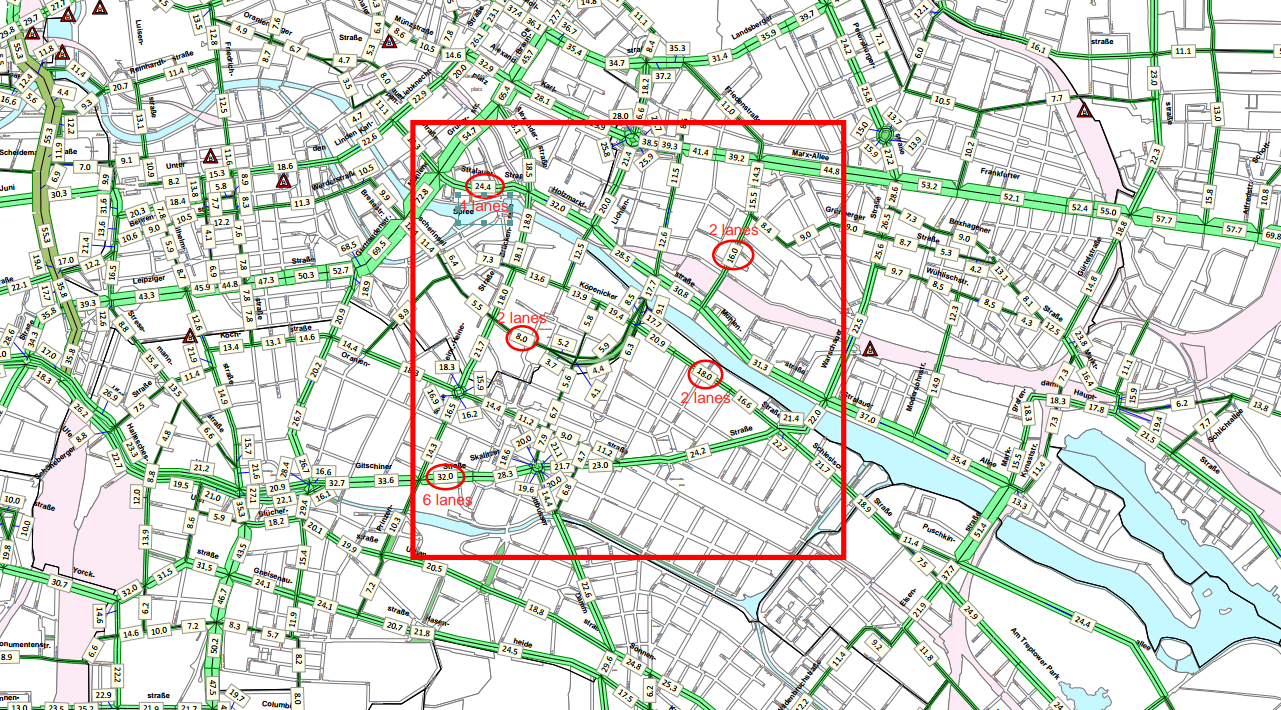
\includegraphics[width=1.0\linewidth]{98_images/berlin_traffic_map_2}
	\caption{Traffic Census Map for Berlin Mitte \cite{VerkehrslenkungBerlinVLB2014}}
	\label{fig:berlin_traffic_map}
\end{figure}

\autoref{fig:berlin_traffic_map} depicts an excerpt from that traffic census map, where the red rectangle marks the \SI{21.25}{\square\km} area used in this evaluation. Red circle indicate five measuring points that were randomly selected for calculation of the average utilization factor. For each of these points a daily vehicle count is given as $N_{i}$ in $\frac{vehicles}{24 h}$, alongside the number of driving lanes $m_i$ at that location.

\begin{gather*}
N_1 = 32,000; \  m_1 = 6 \\
N_2 = 18,000; \  m_2 = 2 \\
N_3 = 16,000; \  m_3 = 2 \\
N_4 = 8,000; \  m_4 = 2 \\
N_5 = 24,000; \  m_5 = 4
\end{gather*}

For more accurate estimation it would have been desirable to have the amount of vehicles per measuring point be modeled as an in-homogeneous Poisson process. However, data is only given in per-day resolution. 

Given the above assumptions for speed, vehicle length and safety distance, the time that one vehicle takes to pass a measurement point can be calculated: $$\Delta t_{pass} = \frac{\SI{0.0162}{\km}}{\SI{24}{\km\per\hour}} = \SI{0.000675}{\hour} = \SI{2.43}{\second}$$

Accordingly, the maximum number of vehicles that can potentially pass a measuring point in 24 hours depend on the number of lanes at that measuring point and is given as: $$N_{pot\_i} = \frac{\SI{24}{\hour}}{\SI{0.000675}{cars\per\hour}} * m_i$$

For every point, its load- or utilization factor can be calculated as the fraction of actually measured cars and maximum potential cars: $$\lambda_i = \frac{N_i}{N_{pot_i}}$$

For the above points it follows
\begin{gather*}
N_{pot\_1} = 213,333; \  \lambda_1 = 15 \% \\
N_{pot\_2} = 71,111; \  \lambda_2 = 25.3 \% \\
N_{pot\_3} = 71,111; \  \lambda_3 = 22.5 \% \\
N_{pot\_4} = 71,111; \  \lambda_4 = 11.25 \% \\
N_{pot\_5} = 142,220; \  \lambda_5 = 16.9 \% \\
\end{gather*}
and an average load factor of $\lambda_{avg} = 18.19 \%$.

It can be concluded that, given the average load factor, an optimistic estimate for the average number of concurrent cars in Berlin Mitte might be given by $$N_{norm} = N_{max} * \lambda_{avg} = \SI[detect-weight]{1109}{cars\per\square\km} * 0.1819 = \textbf{\SI[detect-weight]{202}{cars\per\square\km}}$$.

\subsection{Conclusion}
\label{subsec:problem_analysis:conclusion}
Assuming that all cars were connected and participating in cooperative perception, \textbf{$N_{norm} = \SI[detect-weight]{202}{cars\per\square\km}$} is the amount of vehicles the system should, at minimum, be able to handle. A more pessimistic value, while neglecting the participation of pedestrians and road infrastructure for simplicity, is given by \textbf{$N_{max} = \SI[detect-weight]{1109}{cars\per\square\km}$}.

\section{Goals \& Requirements}
\label{sec:problem_analysis:goals_requirements}
Overall goal of this thesis is to propose, implement and evaluate a cooperative perception system, that facilitates the improvement of connected, autonomous vehicles' average perception quality. However, it is crucial that CP is only to be used as extension for an already working, reliably and secure AD system. \textbf{The presence of cooperative perception must under no circumstances be required for the proper functioning of a self-driving car.}

The presented architecture is supposed to overcome previous systems' limitation discussed in \autoref{sec:problem_analysis:current_limitations} and be able to handle, at minimum, the average expected load determined in \autoref{sec:problem_analysis:traffic_volume_estimation}.

As this work mainly separates into two aspects, we define functional (\textbf{F}) and non-functional (\textbf{NF}) requirements for both parts.

\subsection{Environment Modeling \& State Representation}
\label{subsec:problem_analysis:environment_modeling_state_representation}

Goal is to propose a modeling approach for traffic scenes, that fulfills the following requirements. 

\begin{enumerate}[F1:\ \ ]
	\item \textbf{Expressiveness.} The model should be expressive enough to capture all relevant information about a traffic scene, that is necessary to re-construct it with sufficient precision.
	\item \textbf{Openness.} The model should be open to include information on different levels of abstraction and allow for extension.
\end{enumerate}
\begin{enumerate}[NF1:]
	\item \textbf{Universality.} The model should be universal in such that it is independent of type (e.g. vehicle, pedestrian, RSUs, ...) and sensory of its observer and the involved fusion algorithms.
	\item \textbf{Perspicuity.} The model should be globally valid and understandable, without requiring additional information about the observer.
	\item \textbf{Efficiency.} The model should be efficient in terms of size.
\end{enumerate}

\subsection{Cooperative Perception System}
\label{subsec:problem_analysis:cooperative_perception_system}

Goal is to propose an end-to-end solution for a cooperative perception system architecture and implementation, that fulfills the following requirements. 

\begin{enumerate}[F1:\ \ ]
	\item \textbf{Holism.} The system enable for end-to-end cooperative perception, including message exchange and sensor fusion, for different network patterns, including V2V, V2I and V2P.
	\end{enumerate}
\begin{enumerate}[NF1:]
	\item \textbf{Range.} The system should enable for communication over at least 600 m NLOS.
	\item \textbf{Scalability.} The system should be able to handle at least 202 concurrent network participants per km² (see \autoref{sec:problem_analysis:traffic_volume_estimation}) at a tick rate of 10 Hz (considered sufficient by \cite{Rauch2011, Thandavarayan2019})
	\item \textbf{Efficiency.} The system should aim for low latency and low on-vehicle computation load.
	\item \textbf{Reliability.} The system should avoid to have a single-point-of-failure. 
\end{enumerate}

\section{Scope}
\label{sec:problem_analysis:scope}
As states in \autoref{sec:problem_analysis:goals_requirements}, it is within the scope of this thesis to design a comprehensive proposal, functioning implementation and realistic simulation of cooperative perception..

However, the following is explicitly \textbf{out of scope}.
\begin{itemize}
	\item The implementation does not have the extent and quality of a production-ready, well-tested system.
	\item While the proposed meta model allows for easy extension, for the sake of briefness, it is not complete in a sense that all potentially relevant classes, entities, attributes and relations are specified and implemented.
	\item Any aspects related to security, authentication, data integrity and extensive validation are disregarded.
	\item This thesis does conduct experiments or low-level investigations about 5G-, LTE- or DSRC network characteristics. Existing publications are used for reference instead.
	\item While a working proof-of-concept system is proposed that fulfills the stated requirements (see \autoref{sec:problem_analysis:goals_requirements}), elaborate (performance-related) optimizations of particular aspects (e.g. fusion, message generation, compression, ...) are out of scope.
	\item For the sake of simplicity, only two-dimensional environments are assumed, that is, vertically overlapping road scenes (e.g. with highway bridges) are not supported. However, the system could be extended to do so.
	\item Since detailed, realistic, 3D simulations are used for evaluation, no additional real-world experiments are conducted.
\end{itemize}